\documentclass[12pt]{article}
\usepackage{pgfkeys}
\usepackage[widelayout,sf,ngerman, solution, copyright, hyperref]{custom23}
%\stefancopyright=true
\newcommand{\docName}{Quadratische Funktionen}
%\newcommand{\docVersion}{Parameterform}%Version 1.0.1}
\newcommand{\klasse}{Kantonsschule Wettingen, Klasse G1D}

\fancyhead[L]{\klasse}
\fancyhead[R]{\today}%, \docVersion}
\renewcommand{\headrulewidth}{0.4pt} % Line under the header
\usepackage{wrapfig}

\usepackage{tabularx}
\newcolumntype{Y}{>{\centering\arraybackslash}X}
\renewcommand\tabularxcolumn[1]{m{#1}}% for vertical centering text in X column

\usepackage{makecell}
\usepackage{subcaption}
\setboolean{solution}{true}

\usepackage{soul}
\usepackage{setspace}
\begin{document}
\section{Identifikation Parameter}
\begin{whiteboxdef}
Es seien $A$ und $B$ zwei Teilmengen der reellen Zahlen.

Eine Funktion $f : A \rightarrow B$ heisst \textbf{quadratische Funktion}, wenn drei reelle Konstanten $a,b,c \in \mathbb{R}$ existieren, so dass $a \neq 0$ und so dass gilt:
\begin{IEEEeqnarray}{rClCr}\label{eq:allgemeine_form_quad_func}
f(x) &=& ax^2 + bx + c, &\quad &\forall \; x \in A.
\end{IEEEeqnarray}

Diese Schreibweise für quadratische Funktionen heisst \textbf{allgemeine Form}.
\end{whiteboxdef}


Bestimmen Sie für folgende Funktionsterme die Parameter $a,b,c$, so dass der Funktionsterm die Form $ax^2 + bx + c$ annimmt.

\begin{IEEEeqnarray*}{rCrClCrCrCl}
g &:& \Reals & \rightarrow & \Reals
& \quad &
w &:& \Reals & \rightarrow & \Reals\\
&& x & \mapsto & (x-2)^2 && 
&& x & \mapsto & (x-1)^2 + 3\\
h &:& \Reals & \rightarrow & \Reals
& \quad &
u &:& \Reals & \rightarrow & \Reals\\
&& x & \mapsto & -(x+2)^2 - 5 &&
&& x & \mapsto & 2x^2 + 3
\end{IEEEeqnarray*}


\begin{example}
Der Funktionsterm von $h(x)$ lautet $-(x+2)^2 -5$. Dieser lässt sich wie folgt umformen
\begin{IEEEeqnarray*}{rCl}
-(x+2)^2 - 5 &=& -(x^2 + 4x + 4) - 5\\
&=& -x^2 -4x - 4 - 5\\
&=& -x^2 -4x - 9.
\end{IEEEeqnarray*}
Somit gilt $h(x) = a x^2 + b x + c$, für $a=-1$, $b=-4$ und $c=-9$.
\end{example}
\begin{center}
\begin{tabularx}{0.75\linewidth}{|l|X|X|X|}
\toprule
\textbf{Funktion} & Parameter a & Parameter b & Parameter c\\
\midrule
g & & & \\
& & & \\
\hline
w & & & \\
& & & \\
\hline
h & -1 & -4 & -9\\
& & & \\
\hline
u & & &\\
& & & \\
\bottomrule
\end{tabularx}
\end{center}

\section{Geogebra}
Greifen Sie auf das vorbereitete Geogebra Arbeitsblatt \emph{Parameter} zu.
\begin{figure}[h]
\begin{center}
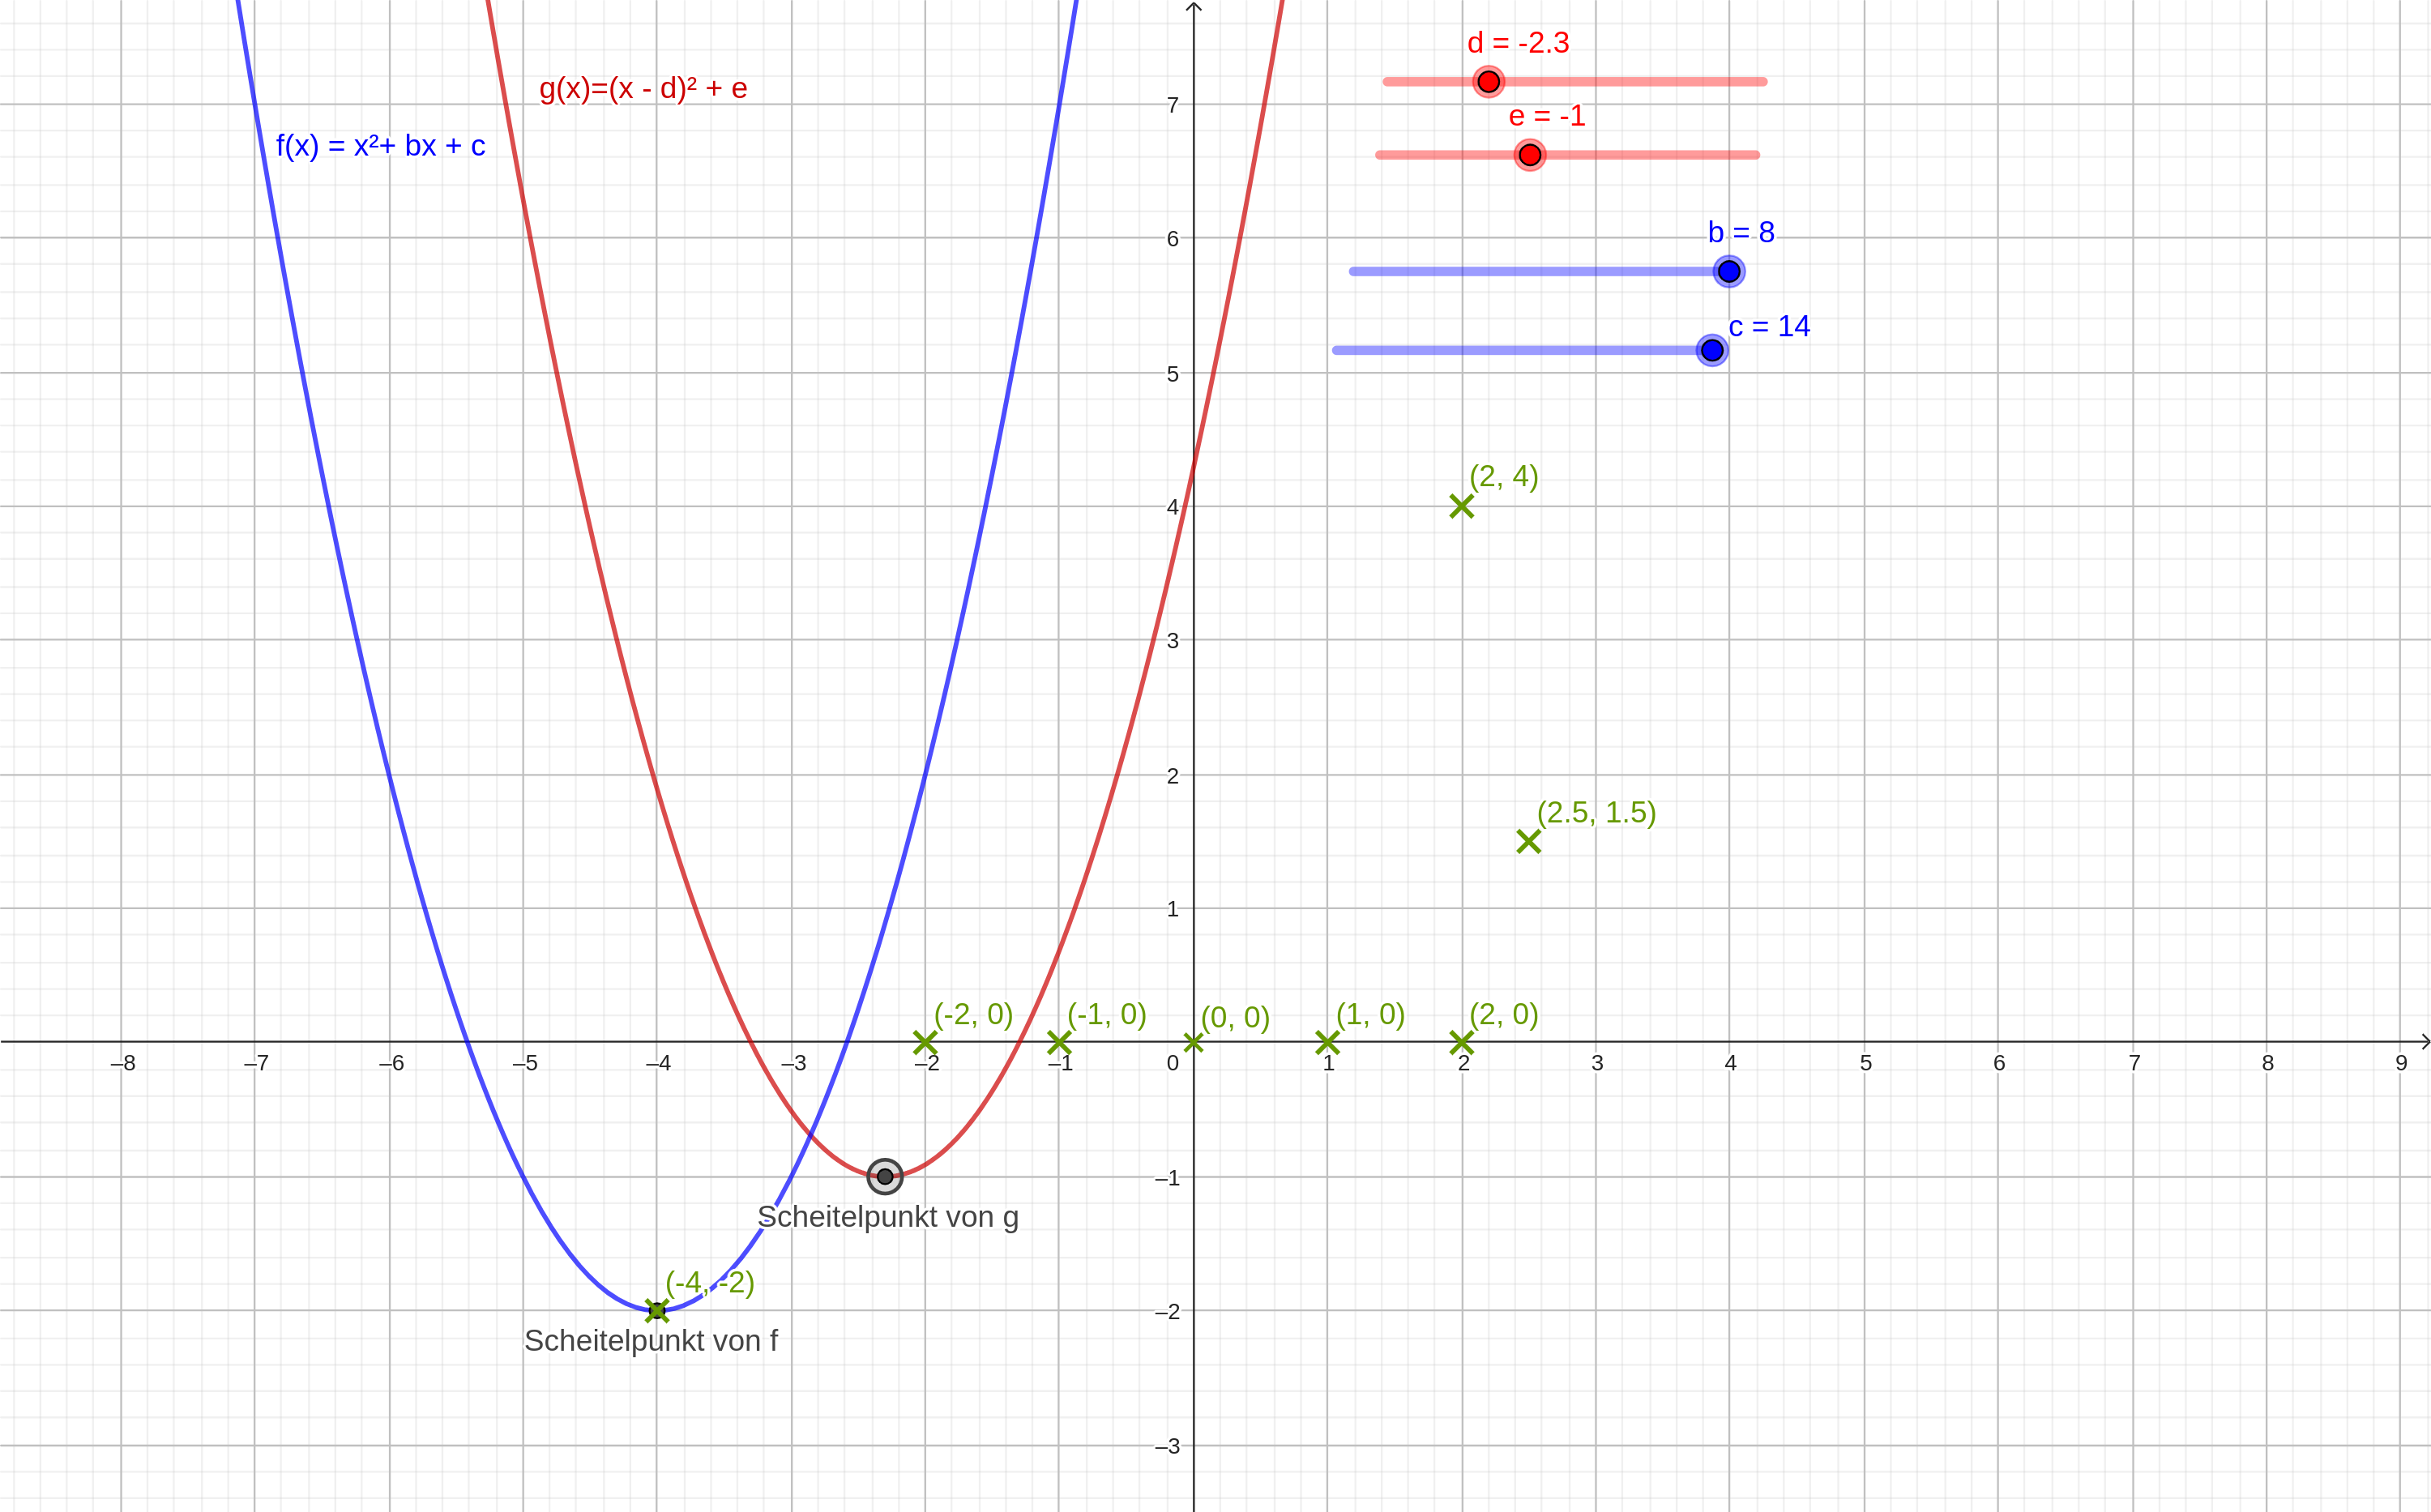
\includegraphics[scale=0.3]{figures/geogebra_thumbnail.png}
\end{center}
\end{figure}

Die blaue Kurve entspricht dem Graphen der parametrisierten Funktion $f$
\begin{IEEEeqnarray*}{rCrCl}
f &:& \Reals &\rightarrow &\Reals\\
&& x & \mapsto & x^2 + bx + c.
\end{IEEEeqnarray*}
Mit den blauen Schiebereglern können Sie die Werte der Parameter $b$ und $c$ verändern.

Die rote Kurve entspricht dem Graphen der parametrisierten Funktion $g$
\begin{IEEEeqnarray*}{rCrCl}
g &:& \Reals &\rightarrow &\Reals\\
&& x & \mapsto  & (x-d)^2 + e.
\end{IEEEeqnarray*}
Mit den roten Schiebereglern können Sie die Werte der Parameter $d$ und $e$ verändern.

Bestimmen Sie die Parameter $b$ und $c$, so dass der Scheitelpunkt von $f$ jeweils auf den grünen Kreuzen zu liegen kommt. Notieren Sie sich die Parameter, die zur gewünschten Konfiguration führen. Machen Sie anschliessend das gleiche für die Funktion $g$, indem Sie die Parameter $d$ und $e$ modifizieren. Halten Sie Ihre Resultate in Tabelle~\ref{tab:params} fest. (Tipp: arbeiten Sie mit anderen Personen zusammen, dann geht es schneller).

\begin{table}\scriptsize
\begin{center}
\begin{tabularx}{0.75\linewidth}{|l|X|X|X|X|}
\toprule 
\textbf{Scheitelpunkt} & \multicolumn{2}{c|}{Funktion $g$} & \multicolumn{2}{c|}{Funktion $f$}\\
& d & e & b & c\\
\midrule
(-4,-2) & -4 & -2 & 8 & 14\\
& & & &\\
\hline
(-2,0) & -2 & 0  & 4  & \\
& & & & \\
\hline
(-1,0) & & & &\\
& & & & \\
\hline
(0,0) & & & &\\
& & & & \\
\hline
(1,0) & & & &\\
& & & & \\
\hline
(2,0) & & & &\\
& & & & \\
\hline
(2,4) & & & &\\
& & & & \\
\hline
(2.5,1.5) & & & &\\
& & & & \\
\bottomrule
\end{tabularx}
\caption{Parameter}\label{tab:params}
\end{center}
\end{table}
\newpage
\section{Der Zusammenhang der Parameter}
Sie haben vielleicht bemerkt, dass die Verschiebung des Funktionsgraphen von $g$ wesentlich einfacher zu verlaufen scheint, als die des Funktionsgraphen von $f$. Wir werden in den folgenden Paragraphen erkennen, dass man quadratische Funktionen mit Funktionsterm $ax^2 + bx + c$ auch als $(x-d)^2 +e$ schreiben kann.
\begin{enumerate}[label=\alph*)]
\item Was ist der Zusammenhang zwischen den Parametern $d,e$ und dem Scheitelpunkt? Welche Werte müssen $d$ und $e$ annehmen, wenn Sie den Scheitelpunkt von $g$ in $(-200, 10)$ positionieren wollten?
\item Sie haben wahrscheinlich bemerkt, dass sich die beiden Funktionen überlagern, wenn Sie den gleichen Scheitelpunkt haben. Können Sie eine Regelmässigkeit in den Parametern $d$ und $b$ erkennen? Vervollständigen Sie folgenden Satz:
\begin{whitebox}\footnotesize
Wenn die quadratischen Funktionen $f: \Reals \rightarrow \Reals, f(x) = x^2 + bx + c$  und $g: \Reals \rightarrow \Reals, g(x) = (x-d)^2 + e$  den gleichen Scheitelpunkt haben, dann ist $b$ gleich \rule{1cm}{0.5pt} mal $d$.
\end{whitebox}
\item Ziehen Sie $e$ von $c$ ab und schreiben Sie den Wert in folgende Tabelle:
{\scriptsize
\begin{tabularx}{\linewidth}{|X|X|X|X|X|X|X|X|X|}
\toprule
&(-4,-2) & (-2,0)& (-1,0)& (0,0)& (1,0) & (2,0) & (2,4) & (2.5,1.5)\\
\midrule
c-e & & & & & & & & \\
& & & & & & & & \\
\bottomrule
\end{tabularx}}\\[1em]
Vervollständigen Sie folgenden Satz:
\begin{whitebox}\footnotesize
Wenn die quadratischen Funktionen $f: \Reals \rightarrow \Reals, f(x) = x^2 + bx + c$  und $g: \Reals \rightarrow \Reals, g(x) = (x-d)^2 + e$  den gleichen Scheitelpunkt haben, dann ist $c-e$ gleich \rule{1cm}{0.5pt}.
\end{whitebox}
\end{enumerate}

\section{Von der Normalform zur Scheitelpunktform}

\begin{enumerate}[label=\alph*)]


%\item Schreiben Sie den Funktionsterm der Funktion $g(x) = (x-d)^2 + e$ aus und bestimmen Sie die Parameter $a,b$ und $c$, so dass $g(x) = ax^2 + bx + c$ gilt (genau so, wie sie das schon in Aufgabe~1 gemacht haben). Vergleichen Sie die Terme mit Ihren Beobachtungen aus Aufgabe~3.
%Vervollständigen Sie folgenden Satz:
%\begin{whitebox}\footnotesize
%Wenn die quadratischen Funktionen $f: \Reals \rightarrow \Reals, f(x) = x^2 + bx + c$  und $g: \Reals \rightarrow \Reals, g(x) = (x-d)^2 + e$  den gleichen Scheitelpunkt haben, dann ist $d$ gleich \rule{1cm}{0.5pt} und $e$ gleich \rule{1cm}{0.5pt}. 
%\end{whitebox}

%Vergleichen Sie die Zuweisungsterme der Funktionen $g$ und $f$:
%\begin{IEEEeqnarray*}{rCrClCrCrCl}
%f &:& \Reals &\rightarrow &\Reals & \qquad & g &:& \Reals &\rightarrow &\Reals\\
%&& x & \mapsto & x^2 + bx + c & \qquad && x & \mapsto  & (x-d)^2 + e.
%\end{IEEEeqnarray*}

\item Nutzen Sie die vorangegangenen Antworten und bestimmen Sie nun die Parameter $d$ und $e$, so dass der Funktionsterm der Funktion $f(x) = x^2 + bx + c$ gleich $(x-d)^2 + e$ ist.

Testen Sie Ihre Formel: es sei $h$ eine quadratische Funktion mit Parameter $a=1, b=2$ und $c=-5.$ Wo liegt ihr Scheitelpunkt? Wenn Sie $(-1, -6)$ erhalten haben, dann scheinen Sie richtig zu liegen. Vervollständigen Sie folgenden Satz:
\begin{whitebox}
Eine quadratische Funktion $f: \Reals \rightarrow \Reals, f(x) = x^2 + bx + c,$ lässt sich auch als $f(x) = (x-d)^2 + e$ schreiben, wobei $d= \rule{1cm}{0.5pt}$ und $e=\rule{1cm}{0.5pt}$ gesetzt wird.\end{whitebox}

\item Wie verhält sich das ganze, wenn jetzt plötzlich der Term $a$ hinzukommt? Wenn also $f(x) = ax^2 + bx + c$ und $g(x) = a(x-d)^2 + e$, mit $a\neq 0$ gilt? Vervollständigen den Satz:

\begin{whitebox}
Eine quadratische Funktion $f: \Reals \rightarrow \Reals, f(x) = ax^2 + bx + c,$ lässt sich auch als $f(x) = a(x-d)^2 + e$ schreiben, wobei $d= \rule{1cm}{0.5pt}$ und $e=\rule{1cm}{0.5pt}$ gesetzt wird.\end{whitebox}
\end{enumerate}


%\label{lastpage}
\end{document}
